\section{Block Diagram}

The picoVersat block diagram is shown in Fig.~\ref{fig:bd}. PicoVersat contains
4 main registers: the accumulator (register A), the data pointer (register B),
the flags register (register C) and the program counter (register PC).

\begin{figure}[!htbp]
    \centerline{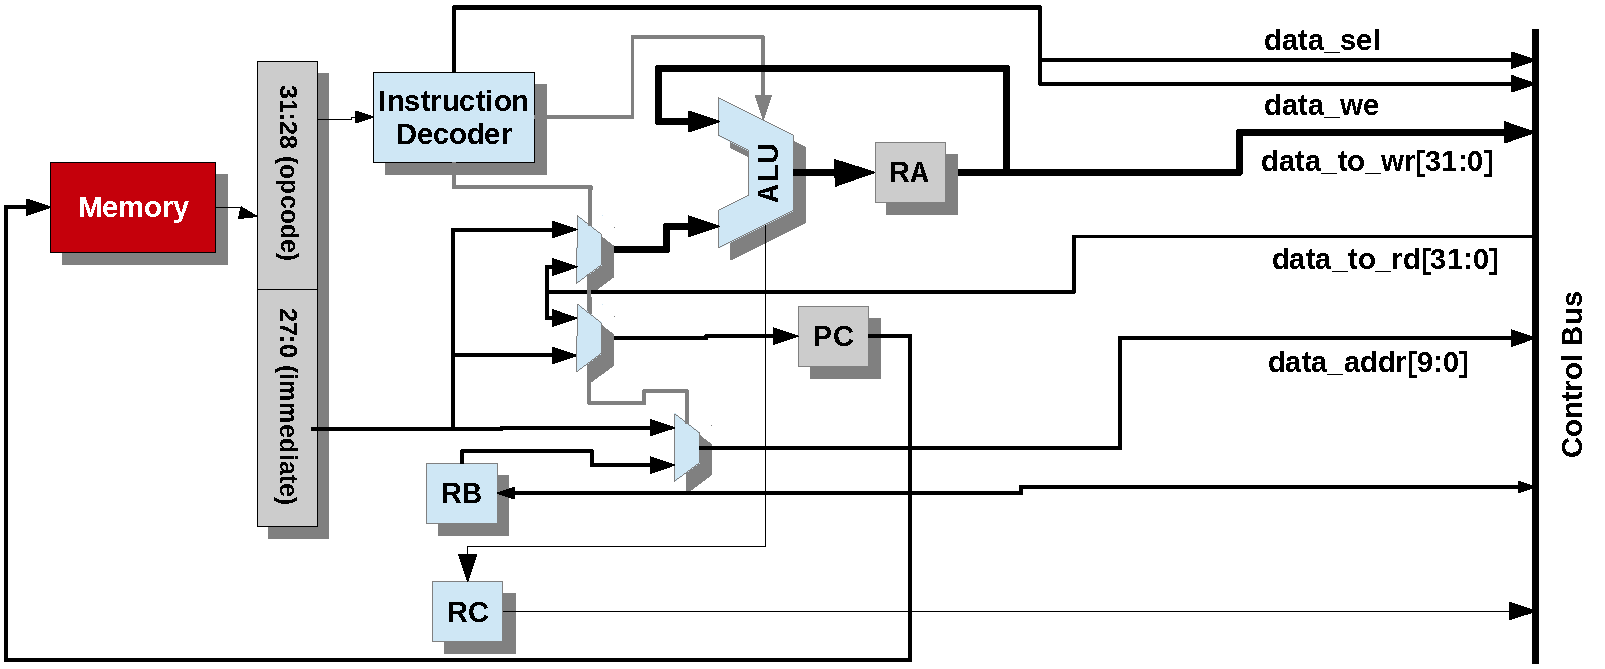
\includegraphics[width=\textwidth]{bd}}
    \vspace{0cm}\caption{Block Diagram}
    \label{fig:bd}
\end{figure}



\subsection{Accumulator register}

Register A, the accumulator, is the main register in this architecture. It can
be loaded with an immediate value from the instruction itself (immediate value)
or with a value read from the data interface. It is the destination of
operations using as operands register A itself and an immediate or addressed
value. Its value is always driven out to the data interface.

\subsection{Pointer register}

Register B, the memory pointer, is used to store the address in indirect loads
and stores to/from the accumulator, respectively, and to store the target
address in branch instructions. Register B itself is in the memory map so it can
be read or written as if accessing the data interface.

\subsection{Flags register}

Register C, the flags register, is used to store three operation flags: the
negative, overflow and carry flags. Register C itself is in the memory map and
it is read-only. The flags are set by the controller ALU and can be read by
programs for decision taking. The structure of register C is shown in
Table~\ref{tab:flags}.

\begin{table}[!htbp]
  \centering
    \begin{tabular}{|c|c|p{7cm}|}
    \hline 
    {\bf Bits} & {\bf Name} & {\bf Description} \\
    \hline \hline 
    31-3 & NA & Reserved for future use\\
    \hline
    2 & Negative & Asserted if last ALU operation generated a negative result\\
    \hline
    1 & Overflow &  Asserted if last ALU operation generated an arithmetic overlow\\
    \hline
    0 & Carry & Asserted if last ALU operation generated a carry\\
    \hline
    \hline

    \end{tabular}
  \caption{Register C: flags}
  \label{tab:flags}
\end{table}


\subsection{PC register}

The Program Counter (PC) register contains the address of the next instruction
to be fetched from the Memory. The PC normally increments to fetch the next
instruction, except for program branch instructions, in which case the PC
register is loaded with the instruction immediate or with the value in register
B, depending on the branch instruction type, direct or indirect, respectively.
